\subsection{Failure Case Analysis}
\label{sec:failure-case-analysis}

While SS-JEPA achieves competitive overall segmentation performance, we observe
failure cases for landslides with small spatial extent. Figure~\ref{fig:failure_cases}
presents representative examples where SS-JEPA tends to miss
localized landslide regions. In terms of per-sample mIoU, I-JEPA exceeds SS-JEPA in approximately 85\% of cases,
with differences ranging from 0.005 to 0.3. This behavior suggests a bias toward
broad spatial patterns in SS-JEPA, where the large number of patch tokens allows
background information to overwhelm sharp, localized details. The linear projection
layer further acts as a bottleneck during multimodal fusion, potentially smoothing
high-frequency spatial signals.

These observations indicate that while spatio-spectral fusion improves the learning
of broader geological structures, it can suppress features with limited spatial
extent. Future work will investigate adaptive weighting mechanisms to preserve such
localized signals during multimodal fusion.


\begin{figure}
	\begin{center}
		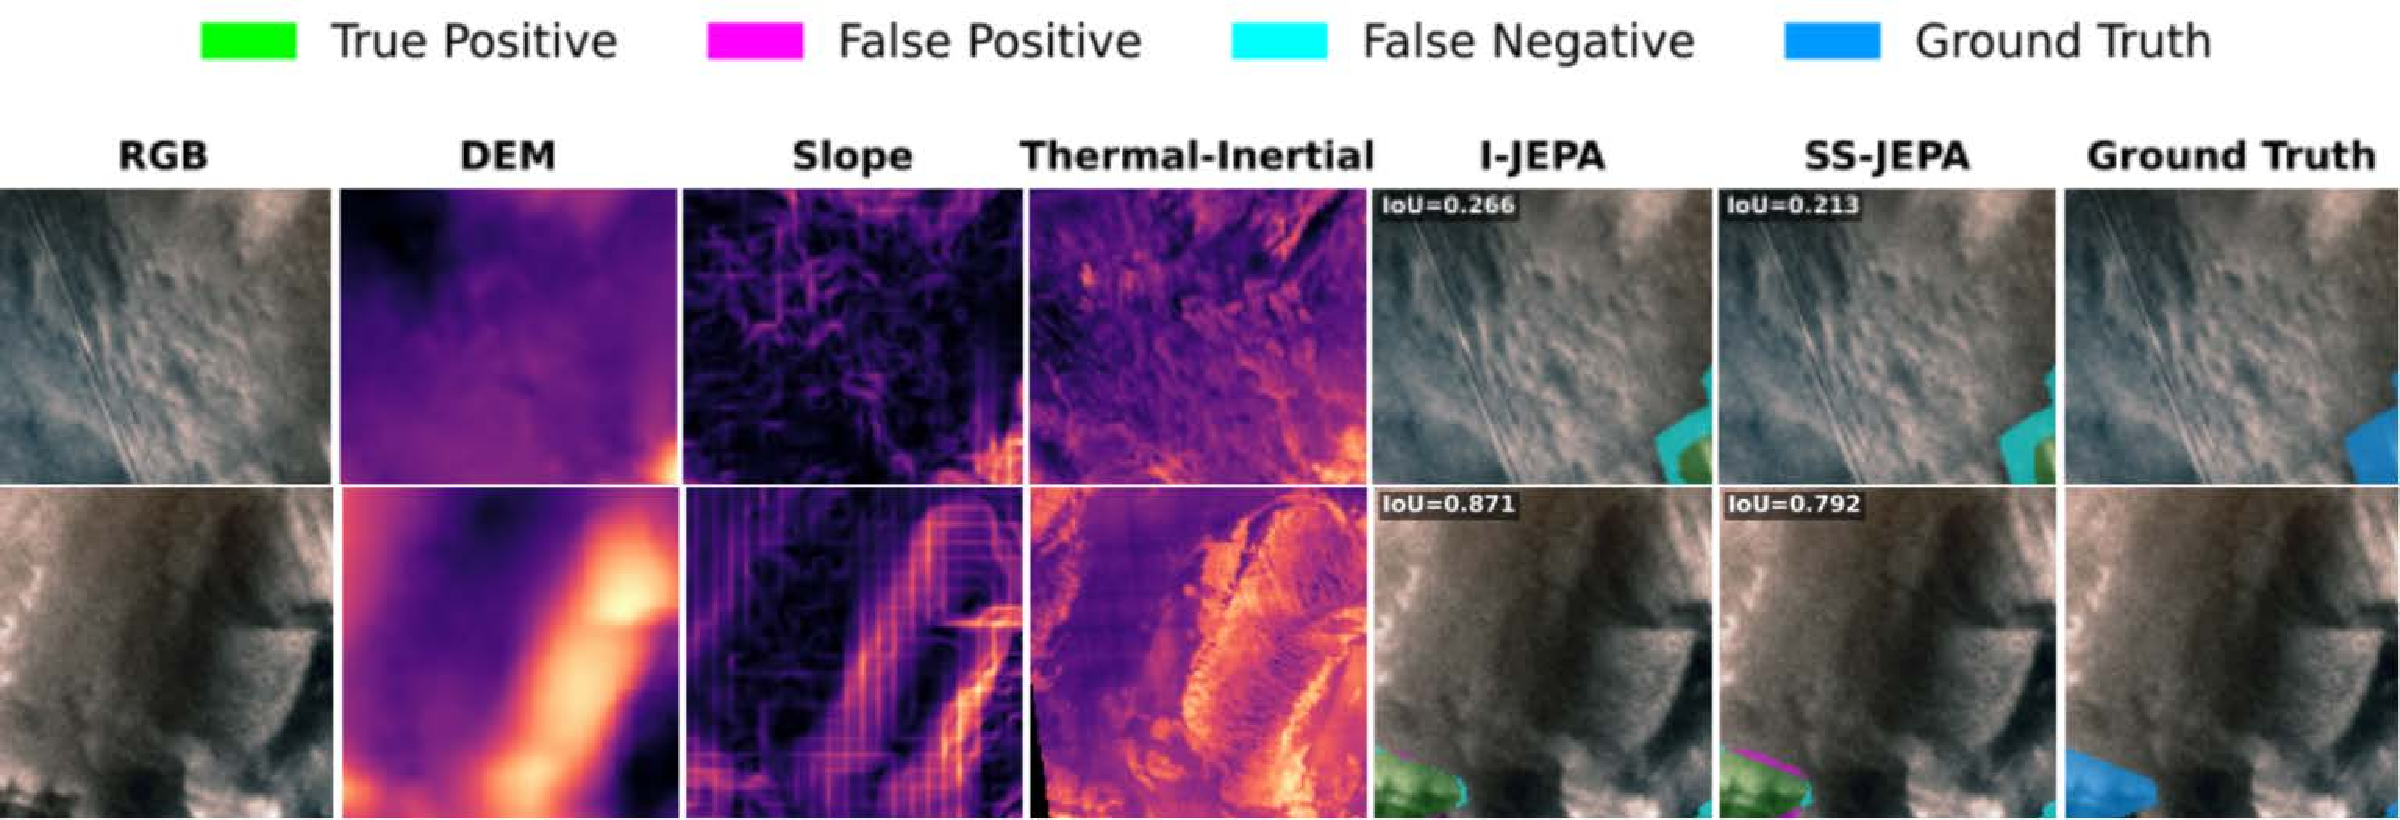
\includegraphics[width=0.65\textwidth]{figures/mar.pdf}
	\end{center}
	\caption{Representative failure cases of SS-JEPA on small spatial-extent landslides compared to I-JEPA.}\label{fig:failure_cases}
\end{figure}